\documentclass[11pt]{article}
\usepackage{amssymb}
\usepackage{amsthm}
\usepackage{enumitem}
\usepackage{amsmath}
\usepackage{bm}
\usepackage{adjustbox}
\usepackage{mathrsfs}
\usepackage{graphicx}
\usepackage{siunitx}

\title{\textbf{Solved selected problems of From Calculus to Chaos - Gregory}}
\author{Franco Zacco}
\date{}

\addtolength{\topmargin}{-3cm}
\addtolength{\textheight}{3cm}

\newcommand{\hatr}{\bm{\hat{r}}}
\newcommand{\hatth}{\bm{\hat{\theta}}}

\begin{document}
\maketitle
\thispagestyle{empty}

\section*{Chapter 3 - Newton's laws of motion and the law of gravitation}

	\begin{proof}{\textbf{3.1}}
        Each mass exerts a gravitational force given by
        $$F = \frac{Gm^2}{a^2}$$
        Given that the masses are all equal and the distance between them is
        $a$, by symmetry we know that the resultant force would be from
        the particle we choose, let's say particle $A$, to the centroid $N$ of the 
        triangle $BCD$. If the angle from the resultant pointing to $N$ to each side of
        the tetrahedron is $\alpha$ then the resultant force is given by
        $$F = \frac{3Gm^2\cos{\alpha}}{a^2}$$
        Let's take the triangle $BCD$, we can form another triangle with the
        line that passes through the centroid of this triangle from particle B
        and generate a triangle $BCN$ where $N$ is a point located in half the
        side from $C$ to $D$ since this is a right triangle by pythagoras we
        have that
        $$BN^2 = BC^2 - CN^2 = a^2 - ( \frac{1}{2}a)^2 = \frac{3}{4}a^2$$
        $$BN = \frac{\sqrt{3}}{2}a$$
        If the centroid is at point $M$ over the line $BN$ then we can
        form a right triangle $BAM$ and again by pythagoras we have that
        \begin{align*}
        AM &= \sqrt{BA^2 - BM^2} \\
           &= \sqrt{BA^2 - (\frac{2}{3}BN)^2} \\
           &= \sqrt{a^2 - (\frac{1}{\sqrt{3}}a)^2} \\
           &= \sqrt{\frac{2}{3}}a
        \end{align*}
        so
        $$\cos{\alpha} = \frac{AN}{BA} = \sqrt{\frac{2}{3}}$$
        and finally we can write $F$ as
        $$F = \frac{\sqrt{6}Gm^2}{a^2}$$
        If now we have a set of spheres placed as a tetrahedron where each centre
        is at a distance $2a$ from the other sphere centres (spheres has radius
        $a$), we have the same problem we solved above since we know that the
        gravitational attraction for spheres can be replaced by the
        gravitational attraction of particles located at the centre of the
        sphere with the same mass as the sphere. Therefore the force exerted on
        the upper sphere is
        $$F = \frac{\sqrt{6}Gm^2}{4a^2}$$
    \end{proof}
	\begin{proof}{\textbf{3.3}}
        Consider the element $[x,x+dx]$ of the rod with mass $Mdx/2a$ then if a
        particle is standing at the point $x=x'$ the element of the rod exerts a
        force to the particle given by
        $$\frac{mMGdx}{2a(x'-x)^2}$$
        but since the rod is a continuous mass we need to sum the force exerted
        to the particle by each element so we must solve the following integral
        \begin{align*}
            F &= \int_{-a}^{a} \frac{mMGdx}{2a(x'-x)^2} \\
              &= \frac{mMG}{2a} \int_{-a}^{a} \frac{dx}{(x'-x)^2} \\
              &= \frac{mMG}{2a} \left[ \frac{1}{x'- x} \right]^{x=a}_{x=-a} \\
              &= \frac{mMG}{2a} \left[ \frac{1}{x'- a} - \frac{1}{x'+ a} \right] \\
              &= \frac{mMG}{2a} \left[ \frac{2a}{(x'- a)(x'+ a)} \right] \\
              &= \frac{mMG}{(x'^2 - a^2)}
        \end{align*}
        Let's now consider the case of the gravitational attraction between two
        rods, consider an element of the second rod $[x', x'+dx']$ which has
        mass $Mdx'/2a$ the force exerted by the first rod to this element is
        then given by replacing $m=Mdx'/2a$ in the equation derivated for a
        particle, so
        $$\frac{(Mdx'/2a)MG}{(x'^2 - a^2)}$$
        but since the second rod is a continuous mass we need to sum the force
        exerted to each element in the rod so we must solve the following
        integral
        \begin{align*}
            F &= \int_{b-a}^{b+a} \frac{M^2Gdx'}{2a(x'^2 - a^2)} \\
              &= \frac{M^2G}{2a} \int_{b-a}^{b+a} \frac{dx'}{(x'^2 - a^2)} \\
              &= \frac{M^2G}{4a^2} \int_{b-a}^{b+a} \left[ \frac{1}{x'- a} - \frac{1}{x'+ a} \right] dx'\\
              &= \frac{M^2G}{4a^2} \left[ \log(x'-a) - \log(x' + a)\right]^{x'=b+a}_{x'=b-a} \\
              &= \frac{M^2G}{4a^2} \left[ \log\left( \frac{x'-a}{x'+a} \right) \right]^{x'=b+a}_{x'=b-a} \\
              &= \frac{M^2G}{4a^2} \left[ \log\left( \frac{b}{b+2a} \right) - \log\left( \frac{b - 2a}{b} \right) \right] \\
              &= \frac{M^2G}{4a^2} \log \left( \frac{b^2}{b^2 - 4a^2} \right) \
        \end{align*}
    \end{proof}
	\begin{proof}{\textbf{3.4}}
        From the already obtained equation for the force exerted by a disk of
        mass $M$ on a particle P of mass $m$ we can determine the force exerted
        by the disk on a rod of mass $M'$ by considering an element of the rod,
        $[x,x+dx]$ of mass $m=M'dx/b$ then if this element is at a distance $x$
        from the axis of symmetry of the disk, the force exerted on the element
        by the disk is therefore
        $$\frac{2M'MG}{a^2b} \left[ 1 - \frac{x}{\sqrt{a^2 + x^2}} \right]dx$$
        Since the rod is a continuous mass we need to sum every element of the
        rod by integration, since the rod has length $b$ then the integration
        limits are $0 \leq x \leq b$.
        \begin{align*}
            F &= \int_0^{b} \frac{2M'MG}{a^2b} \left[ 1 - \frac{x}{\sqrt{a^2 + x^2}} \right]dx \\
              &= \frac{2M'MG}{a^2b} \int_0^{b} \left[ 1 - \frac{x}{\sqrt{a^2 + x^2}} \right]dx \\
              &= \frac{2M'MG}{a^2b} \left[\int_0^{b} dx - \int_0^{b} \frac{xdx}{\sqrt{a^2 + x^2}} \right]
        \end{align*}
        The second integral can be solved by substitution if $t = a^2 + x^2$
        so $dt = 2x dx$ and then
        \begin{align*}
            \int \frac{xdx}{\sqrt{a^2 + x^2}} &= \int \frac{dt}{2 \sqrt{t}} \\
                &= \sqrt{t} \\
                &= \sqrt{a^2 + x^2}
        \end{align*}
        Finally we have that
        \begin{align*}
            F &= \frac{2M'MG}{a^2b} \left[ \left[ x \right]_{x=0}^{x=b} - [\sqrt{a^2 + x^2}]_{x=0}^{x=b} \right] \\
              &= \frac{2M'MG}{a^2b} \left[ [b - 0] - [\sqrt{a^2 + b^2} - \sqrt{a^2}] \right] \\
              &= \frac{2M'MG}{a^2b} \left[ b + a - \sqrt{a^2 + b^2} \right]
        \end{align*}
    \end{proof}
	\begin{proof}{\textbf{3.5}}
        When a particle is inside a hollow symmetric sphere the distance
        between the origin and the particle is less than the distance from the
        origin to a slected element in the sphere, meaning that $b < r$. So now
        $R$ which is the distance from the particle to the element we selected
        from the hollow sphere can vary as $r-b \leq R \leq r+b$.\\
        So following the proof we already have when we need to do the
        $\theta$-integration we change variables to do an $R$-integration so
        we are left with the following integral where we have changed the
        integration bounds.
        \begin{align*}
            \int_{r-b}^{r+b} \left( 1 + \frac{b^2 - r^2}{R^2} \right) dR \ 
                &= \left[R - \frac{b^2 - r^2}{R} \right]_{R=r-b}^{R=r+b} \\
                &= \left[ [(r+b) - (r-b)] - (b^2 - r^2)\left[ \frac{1}{r+b} - \frac{1}{r-b} \right] \right] \\
                &= \left[ 2b - (b^2 - r^2) \left[ \frac{(r-b) - (r+b)}{(r^2 - b^2)} \right] \right] \\
                &= \left[ 2b + \left[(r-b) - (r+b)\right] \right] \\
                &= 0
        \end{align*}
        Therefore the force exerted by the hollow sphere to the particle inside
        is 0.
    \end{proof}
	\begin{proof}{\textbf{3.6}}
        Given that we can assume that the hole is narrow and can be ignored if
        we separate the sphere in different shells where there is a shell that
        extends from $a-r$ to $a$ then the particle would be in the inside of 
        this shell which forms what we know as a hollow sphere with the
        particle inside, therefore the force exerted by this shell to the
        particle is 0. \\
        On the other hand, we are left with the shell that extend to the origin
        of the sphere which means that the particle is having a force exerted
        to it by an external solid sphere with radius $r$ and mass $M(r/a)^3$.\\
        Therefore the force exerted to the particle is the same as if in the
        origin we had a particle of mass $M(r/a)^3$ then
        \begin{align*}
            F &= \frac{mM(r/a)^3G}{r^2} \\
              &= \frac{mMGr}{a^3}
        \end{align*}
    \end{proof}
	\begin{proof}{\textbf{3.9}}
        Let's consider an element of the wire with a mass of $M d\theta/2\pi a$
        so the force exerted to the particle which is in the plane of the wire
        is
        $$\frac{m(M d\theta/2\pi a)G}{R^2}$$
        where $a$ is the radius of the circle formed with the wire and $R$ is
        the distance between the element selected in the wire and the particle.
        Since the wire is a continuous mass we should sum the force exerted by
        every element by integration taking into account that the resultant
        force exerted will be in the PO direction so
        \begin{align*}
            F &= \frac{mMG}{2\pi a} \int_0^{2\pi}{\frac{\cos{\alpha}}{R^2}}d\theta \\
              &= \frac{mMG}{2\pi a} \int_0^{2\pi}{\frac{R\cos{\alpha}}{R^3}}d\theta
        \end{align*}
        By the cosine rule we also have that $R^2 = a^2 + b^2 - 2ba\cos{\theta}$\\
        also $R\cos{\alpha} = a - b\cos{\theta}$ so replacing we have that
        \begin{align*}
            F &= \frac{mMG}{2\pi a} \int_0^{2\pi}{\frac{a - b\cos{\theta}}{(a^2 + b^2 - 2ba\cos{\theta})^{3/2}}}d\theta \\
              &= \frac{mMG}{2\pi a} \int_0^{2\pi}{\frac{a(1 - b/a\cos{\theta})}{(\sqrt{a^2(1 + b^2/a^2 - 2ba/a^2 \cos{\theta})})^{3}}}d\theta \\
              &= \frac{mMG}{2\pi a} \int_0^{2\pi}{\frac{a(1 - b/a\cos{\theta})}{a^3(\sqrt{1 + b^2/a^2 - 2ba/a^2 \cos{\theta}})^{3}}}d\theta \\
              &= \frac{mMG}{2\pi a^3} \int_0^{2\pi}{\frac{1 - \xi\cos{\theta}}{(1 + \xi^2 - 2\xi\cos{\theta})^{3/2}}}d\theta
        \end{align*}
\cleardoublepage
        Using computer assistance to integrate the equation (the simpson's
        method), we obtained the following graph for $F$ as $\xi$ changes. \\
        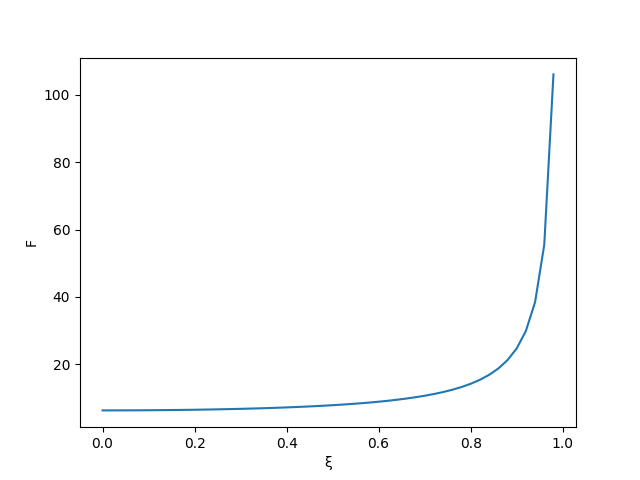
\includegraphics{gregory-3.9.png}
        Finally, as we noticed if $\xi = 0$ the center is not stable because the
        force is not null, then if we assume that Saturn is a sphere then it
        can be replaced by a particle with the same mass located at the center
        of the sphere, if the rings were solid the center would not be a stable
        point, therefore the rings are not solid.
    \end{proof}

\end{document}























